\documentclass[compress]{beamer}

%%%%% PREAMBLE %%%%%

% we want to draw diagrams (turns out not like this though)
\usepackage{tikz}

% figures in a presentation look better without "Figure"
\usepackage{caption}
\captionsetup[figure]{labelformat=empty}

% for Idris syntax highlighting
\usepackage{idrislang}

%%%%% TODO: REMOVE ME!!! %%%%%
\usepackage{todonotes}
\setuptodonotes{inline} % for things to work nicely with beamer
%%%%% TODO: REMOVE ME!!! %%%%%

%\usetheme{Zurich}  % doesn't work for some reason
%\usetheme{Flip}
\usetheme{metropolis}

\title{Degrees of Software Correctness}
\subtitle{Uniting the Spectrum of Verification}

\author{Thomas Ekstr{\" o}m Hansen}
\date{10\textsuperscript{th} November 2023}

\definecolor{staBlue}{HTML}{00539b}
%\definecolor{staMidGreen}{HTML}{00853f}
\definecolor{staDarkGreen}{HTML}{005953}
\setbeamercolor{frametitle}{bg=staDarkGreen}


%%%%% DOCUMENT %%%%%

\begin{document}

\maketitle

\begin{frame}
  \frametitle{Introduction}

  \begin{itemize}
    \item We generally want software to be correct
    \item Many approaches to this
      \begin{itemize}
        \item Test Driven Development (TDD)
        \item Mutation testing
        \item Property-based testing
        \item Model Checking
        \item Type theory
        \item Mathematical abstractions and proofs
      \end{itemize}
    \item No one-size-fits-all
      \begin{itemize}
        \item So compromises are made
      \end{itemize}
  \end{itemize}

\end{frame}

\begin{frame}
  \frametitle{Spectrum of Verification}
  %\todo{Line with arrows detailing downsides?}

  % ~~probably~~ definitely cursed
  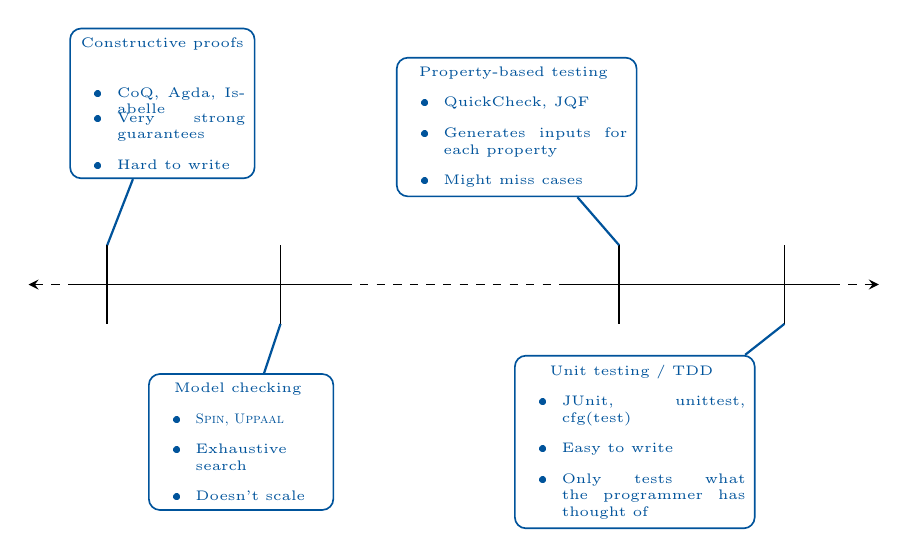
\begin{tikzpicture}[> = stealth, semithick]
    % scale %

    % left half
    \draw [dashed, <-] (-0.2, 0) -- (0.4, 0) ;
    \draw (0.4, 0) -- (3.8, 0) ;

    % middle dashed
    \draw [dashed] (3.8, 0) -- (6.6, 0) ;

    % right half
    \draw (6.6, 0) -- (10, 0) ;
    \draw [dashed, ->] (10, 0) -- (10.6, 0) ;


    % ticks / vertical lines %

    % leftmost tick (constructive proofs)
    \draw (0.8, -0.5) -- (0.8, 0.5) ; %node [above right] {\small Formal proofs};
    
    % tick for model checking
    \draw (3, -0.5) -- (3, 0.5) ;

    % tick for Quickcheck
    \draw (7.3, -0.5) -- (7.3, 0.5) ;

    % rightmost tick (unit tests)
    \draw (9.4, -0.5) -- (9.4, 0.5) ; %node [above left] {\small Unit tests};


    % text boxes with arrows %

    % constructive proofs
    \node [draw, rounded corners,
          text width=6em,
          align=flush center,
          color=staBlue]% 
          at (1.5, 2.3)
          (tbox-prf)
          \bgroup
          \tiny
          Constructive proofs
          \vspace*{-2pt}
          % LaTeX looks beautiful and nice
          % Also LaTeX:
          \setlength{\leftmargini}{2em}
          \begin{itemize}%[leftmargin=*]
            \item CoQ, Agda, Isabelle \vspace*{-11pt}
            \item Very strong guarantees \vspace*{-3pt}
            \item Hard to write
          \end{itemize}
          \egroup
          ;
    \draw [thick, color=staBlue] (tbox-prf) -- (0.8, 0.5) ;

    % model checking
    \node [draw, rounded corners,
          text width=6em,
          align=flush center,
          color=staBlue]% 
          at (2.5, -2)
          (tbox-mc)
          \bgroup
          \tiny
          Model checking
          \vspace*{-3pt}
          \setlength{\leftmargini}{2em}
          \begin{itemize}%[leftmargin=*]
            \item \textsc{Spin, Uppaal}  \vspace*{-3pt}
            \item Exhaustive search  \vspace*{-3pt}
            \item Doesn't scale
          \end{itemize}
          \egroup
          ;
    \draw [thick, color=staBlue] (tbox-mc) -- (3, -0.5) ;

    % property-based testing
    \node [draw, rounded corners,
          text width=8em,
          align=flush center,
          color=staBlue]% 
          at (6, 2)
          (tbox-qc)
          \bgroup
          \tiny
          Property-based testing
          \vspace*{-3pt}
          \setlength{\leftmargini}{2em}
          \begin{itemize}%[leftmargin=*]
            \item QuickCheck, JQF \vspace*{-3pt}
            \item Generates inputs for each property \vspace*{-3pt}
            \item Might miss cases
          \end{itemize}
          \egroup
          ;
    \draw [thick, color=staBlue] (tbox-qc) -- (7.3, 0.5) ;

    % tdd
    \node [draw, rounded corners,
          text width=8em,
          align=flush center,
          color=staBlue]% 
          at (7.5, -2)
          (tbox-tdd)
          \bgroup
          \tiny
          Unit testing / TDD
          \vspace*{-3pt}
          \setlength{\leftmargini}{2em}
          \begin{itemize}%[leftmargin=*]
            \item JUnit, unittest, cfg(test) \vspace*{-3pt}
            \item Easy to write \vspace*{-3pt}
            \item Only tests what the programmer has thought of
          \end{itemize}
          \egroup
          ;
    \draw [thick, color=staBlue] (tbox-tdd) -- (9.4, -0.5) ;

  \end{tikzpicture}

\end{frame}

\begin{frame}
  \frametitle{The eternal problem with verification systems}

  \begin{itemize}
    \item All verification systems face the same problem: ergonomics
    \item If the system is not unobtrusive, people are unlikely to use it
    \item Our hope is that our approach tries to not get in the way by being
          part of the program
      \begin{itemize}
        \item Compiler and type-system assist you rather than hinder
        \item Verify as you go along, tuning the strictness as necessary
        \item Escape hatches provided for prototyping
      \end{itemize}
  \end{itemize}

\end{frame}

\begin{frame}
  \frametitle{Visuals can really help}
  
  %\todo{ATM-dot, ISM, links between them}

  \begin{center}
  \begin{figure}
    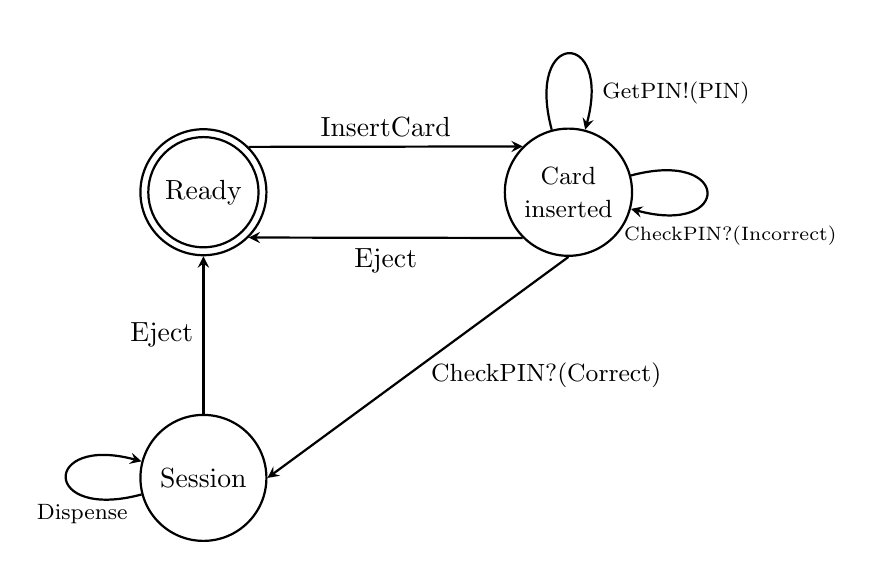
\begin{tikzpicture}[> = stealth, thick,
                        roundnode/.style={circle, draw=black!100, minimum size=16mm},
                        node distance=2cm and 3cm]
      % ATM states %
      \node [circle, draw=black!100, minimum size=14mm] {} ;
      \node[roundnode] (st-ready) {Ready} ;
      \node[roundnode] (st-card) [right=of st-ready, align=center] {\small Card\\\small inserted} ;
      \node[roundnode] (st-session) [below=of st-ready] {Session} ;

      % Arrows %
      \draw [->] (st-ready.north east) -- (st-card.north west)
            node [above, midway] {InsertCard} ;

      \draw [->] (st-card.south west) -- (st-ready.south east)
            node [below, midway] {Eject} ;
      \draw [->] (st-card.south) -- (st-session.east)
            node [right, midway, xshift=1pt, yshift=-1mm] {\small CheckPIN?(Correct)} ;

      \draw [->] (st-session.north) -- (st-ready.south)
            node [left, midway] {Eject} ;

      % Lööps %
      \draw [->] (st-card) to[loop above]
            node [right, xshift=3mm, yshift=-5mm] {\footnotesize GetPIN!(PIN)}
            () ;
      \draw [->] (st-card) to[loop right]
            node [below, xshift=3mm, yshift=-3mm] {\scriptsize CheckPIN?(Incorrect)}
            () ;
      \draw [->] (st-session) to[loop left]
            node [below, xshift=2mm, yshift=-2mm] {\footnotesize Dispense} () ;
    \end{tikzpicture}

    \caption{State machine of an ATM}
  \end{figure}
  \end{center}

\end{frame}

\begin{frame}
  \frametitle{Using types only gets you part of the way there}

  % TODO: try to get this nicer via Katla?
  \vspace*{-3mm}
  \idrisinput{ATM.idr}
\end{frame}

\begin{frame}
  \frametitle{Benefits of a multifaceted approach}

  \begin{enumerate}
    \item Adaptability {\textemdash} right tool for the job
    \item Speed {\textemdash} can trade speed for level of verification
    \item \textbf{Coherence} {\textemdash} all done in one system
      \begin{itemize}
        \item No need to translate to model-checking tool
        \item Specification lives alongside model lives alongside
              implementation
        \item Parts can be verified independently \emph{while} combining into an
              overall system
      \end{itemize}
  \end{enumerate}

\end{frame}

\begin{frame}
  \frametitle{Example: ARQ {\textendash} overview}

  \todo{Rework this slide; protocol diagram?}
  \todo{Different parts necessitate different amounts of verification}

  \begin{itemize}
    \item Automated Repeat reQuest {\textcolor{white}{(of course -\_-)}}
    \item Sender sends one packet at a time
    \item Wait for the receiver to acknowledge them
    \item Resend if no ack is received within a given timeout
  \end{itemize}

  \begin{itemize}
    \item Infinite states
    \item Interface outwith our control
    \item Other half possibly outwith our control
  \end{itemize}

\end{frame}

\begin{frame}
  \frametitle{Conclusion}

  \begin{itemize}
    \item Many verification tools exist, none of them cover enough on their own
    \item Instead of ``competing'', combine the systems to work together
    \item Hopefully this will lead to wider adoption and better whole-system
          soundness
  \end{itemize}

\end{frame}

\begin{frame}
  \frametitle{Questions}

  \begin{center}
    \textcolor{orange}{\Large Questions?}
  \end{center}

\end{frame}

\end{document}